
%-----------------------------------------------------------------------------------------------------
%%  نمایه و واژه‌نامه‌های فارسی به انگلیسی و انگلیسی به فارسی با استفاده از xindy تولید می‌شوند.
%%  برای تولید این بخش‌ها ابتدا با دنبال کردن فرآیند زیر فرمان مناسب را در TexMaker تعریف کنید:
%%  از منوی User گزینهٔ User Commands و سپس Edit User Commands را انتخاب کنید. در جعبه Menu Item عبارت Xindy و در جعبه %%  Command  دستور زیر را قرار دهید (توجه کنید که علامت %  در ابتدای خط جزو دستور نیست) و OK را کلیک کنید
% xindy -L persian-variant2 -C utf8 -I  xindy -M %.xdy -t %.edic -o %.edics %.edico  | xindy -L persian-variant2 -C utf8 -I  xindy -M %.xdy -t %.fdic -o %.fdics %.fdico
%% با توجه به فایل نمونه از دستورات inpdic، indic و inind برای اضافه کردن لغات به نمایه یا واژه‌نامه استفاده کنید.
%% برای مشاهده نمایه و واژه‌نامه ابتدا Quick Build و پس از تکمیل اجرای آن از منوی User گزینه User Commands و سپس Xindy را اجرا کنید. بعد از آن دوباره Quick Build را دو بار اجرا کنید.


\def\sseq{\subseteq}
\def\BB{\mathbb{B}}
\def\st{s. t.}
\def\by{{\boldsymbol y}}
\def\bz{{\boldsymbol z}}
\def\bx{{\boldsymbol x}}
\def\bu{{\boldsymbol u}}
\def\bv{{\boldsymbol v}}

% اگر از تنظیم draftmode استفاده کنید صفحه‌های مربوط به تقدیم، تشکر و جدول مشخصات پایان‌نامه/رساله نمایش داده نمی‌شود. برای تولید نسخهٔ نهایی draftmode را حذف کنید.
%% تنظیم phd و msc به ترتیب برای تولید رساله و پایان‌نامه به کار می‌روند.
\documentclass[msc]{AlzahraThesis}

%% نسخهٔ نهایی برای ارائه به کتابخانه
%\documentclass[phd]{AlzahraThesis}
% بسته‌های مورد نیاز خود را در این بخش usepackage کنید.

% از بسته ptext برای تولید متن تصادفی فارسی استفاده می‌شود (هنگام نگارش پایان‌نامه این بسته را غیرفعال کنید).
\usepackage{ptext}
% از بسته tikz برای رسم گراف استفاده می‌شود (هنگام نگارش پایان‌نامه در صورتی که رسم گراف ندارید، این دستور را غیرفعال کنید).
\usepackage{tikz}

% دستور و تنظیمات مربوط به بسته xepersian (این بخش را تغییر ندهید)
\usepackage[extrafootnotefeatures]{xepersian}
\settextfont[Scale=1.1]{XB Zar}
\setdigitfont[Scale=1]{XB Yas}

\defpersianfont\chapternumber[Scale=3]{XB Zar}
\defpersianfont\chapterfont[Scale=2]{XB Zar}
\defpersianfont\sectionfont[Scale=1.1]{XB Zar}
\defpersianfont\subsectionfont[Scale=1]{XB Zar}
\twocolumnfootnotes





%%  در این بخش می‌توانید صفحه تقدیر و تشکر را به کلاس معرفی کنید. اگر آن را کامنت کنید این صفحه در خروجی نمایش داده نمی‌شود.
\acknowledgment{
%
%\newpage

سپاس گزاری\\

توضیح: این صفحه برای سپاسگزاری دانشجو از افراد یا سازمان ها در نظر گرفته‌ شده است. اگر از کسی سپاسگزاری نمی‌شود، لطفاً این صفحه را پاک کنید.
}
%% در این بخش می‌توانید صفحه تقدیم را به کلاس معرفی کنید. اگر آن را کامنت کنید این صفحه در خروجی نمایش داده نمی‌شود.
\dedication{



\vspace{4cm}

%{\nastaliq%
{\Huge
 تقدیم به همه آنهایی که 
\vspace{1.5cm}

\hspace{3cm}
می خواهند بیشتر بدانند
}

}

%% در این بخش مشخصات پایان‌نامه به کلاس معرفی می‌شود. فایل specifications را مشابه نمونه داده شده و مطابق با
%% رساله/پایان‌نامه خود ویرایش کنید.
% در این فایل، عنوان پایان‌نامه، مشخصات خود، متن تقدیمی‌، ستایش، سپاس‌گزاری و چکیده پایان‌نامه را به فارسی، وارد کنید.
% توجه داشته باشید که جدول حاوی مشخصات پروژه/پایان‌نامه/رساله و همچنین، مشخصات داخل آن، به طور خودکار، درج می‌شود.
%%%%%%%%%%%%%%%%%%%%%%%%%%%%%%%%%%%%
% دانشگاه خود را وارد کنید
\university {الزهراء(س)}
% دانشکده، آموزشکده و یا پژوهشکده  خود را وارد کنید (به فارسی و انگلیسی).
\faculty{ دانشکده علوم ریاضی}
\enfaculty{Mathematical Sciences}

% گروه آموزشی خود را وارد کنید (به فارسی و انگلیسی).
\department{ریاضی  }
\endepartment{Mathematics}


% گروه آموزشی خود را وارد کنید (به فارسی و انگلیسی).
\subject{ریاضی کاربردی}
\ensubject{Applied Mathematics}

% گرایش خود را وارد کنید (به فارسی و انگلیسی). در صورتی که فقط رشته تحصیلی دارید مانند رشته بیوانفورماتیک باید این دستور را با قرار دادن علامت % قبل از آن غیر فعال کنید.
\field{بهینه‌سازی} 
\enfield{Optimization}

% عنوان پایان‌نامه را وارد کنید (به فارسی و انگلیسی).
\title{
نوشتن پروژه، پایان‌نامه و رساله با استفاده از کلاس 
\lr{AlzahraThesis} 
}
\entitle{Writing projects, theses and dissertations using Alzahra\_thesis Class}

% نام استاد(ان) راهنما را وارد کنید (به فارسی و انگلیسی).
\firstsupervisor{فرید بهروزی}
\enfirstsupervisor{Farid Behrouzi}

% وابستگی سازمانی استاد راهنمای اول را وارد کنید. توجه کنید که وابستگی سازمان در قالب زیر بیان شود:
% گروه، دانشکده، دانشگاه، شهر، کشور
\firstsupervisoraffiliation{%
گروه ریاضی، دانشکده علوم ریاضی، دانشگاه الزهرا (س)، تهران، ایران
}
\enfirstsupervisoraffiliation{%
Department of Mathematics, Faculty of Mathematical Sciences, Alzahra Univesrity, Tehran, Iran
}

\secondsupervisor{ابولقاسم لاله}
\ensecondsupervisor{Abolghasem Laleh}

\secondsupervisoraffiliation{%
گروه ریاضی، دانشکده علوم ریاضی، دانشگاه الزهرا (س)، تهران، ایران
}
\ensecondsupervisoraffiliation{Department of Mathematics, Faculty of Mathematical Sciences, Alzahra Univesrity, Tehran, Iran
}



% نام استاد(دان) مشاور را وارد کنید. چنانچه استاد مشاور ندارید، دستور پایین را غیرفعال کنید.
\firstadvisor{علیمردان شاهرضایی}
\enfirstadvisor{Alimardan Shahrezaee}

\firstadvisoraffiliation{%
گروه ریاضی، دانشکده علوم ریاضی، دانشگاه الزهرا (س)، تهران، ایران
}
\enfirstadvisoraffiliation{Department of Mathematics, Faculty of Mathematical Sciences, Alzahra Univesrity, Tehran, Iran
}

\secondadvisor{کامران دیوانی آذر}
\ensecondadvisor{Kamran Divaniazar}

\secondadvisoraffiliation{%
گروه ریاضی، دانشکده علوم ریاضی، دانشگاه الزهرا (س)، تهران، ایران
}
\ensecondadvisoraffiliation{Department of Mathematics, Faculty of Mathematical Sciences, Alzahra Univesrity, Tehran, Iran
}



% نام پژوهشگر را وارد کنید
\name{احسان}
\enname{Sayyed Ehsan}
% نام خانوادگی پژوهشگر را وارد کنید
\surname{منبتی}
\ensurname{Monabbati}

% تاریخ پایان‌نامه را وارد کنید
\thesisdate{ فروردین‌ماه ۱۳۹۵}
\enthesisdate{March, 2011 }

% کلمات کلیدی پایان‌نامه را وارد کنید
\keywords{بهینه‌سازی نامقید، روش گرادیان مزدوج}
\enkeywords{Probabilistic powerdomain; Stably compact space; Valuation}


% چکیده پایان‌نامه را وارد کنید
\faAbstract{
 چکیده می­تواند 250 تا 300 واژه داشته باشد و باید در یک صفحه گنجانده شود. در نگارش چکیده جمله‌های کامل (فعل‌دار) به‌کار می‌روند. چکیده شامل هدف، روش­شناسی پژوهش، یافته­ها، نتیجه‌گیری وکلیدواژه­ها است. در چکیده، بیشتر جمله‌های معلوم به‌جای جمله‌های مجهول می‌آیند. در چکیده فرمولی نوشته نمی‌شود ولی اگر نیاز باشد باید واژه‌های فارسی برای نوشتن آن به‌کار روند. در متن چکيده، از ارجاع به منابع و اشاره به جداول و نمودارها اجتناب شود. در پایان‌نامه/ رساله­هایی که متن اصلی آن‌ها به زبان فارسی است، نخست چکیده فارسی و در پایان نیز چکیده به زبان انگلیسی می‌آید، پایان­نامه/ رساله­هایی که به سایر زبان­ها (عربی، فرانسه و...) نوشته می‌شوند، چکیده باید به سه زبان، 1- زبان فارسی (برای خواننده‌های فارسی‌زبان)، 2- سایر زبان‌های عربی و فرانسه و ... (برای خواننده‌های عربی زبان، فرانسه زبان و ...)، 3- زبان انگلیسی نوشته شود. همچنین ترتیب قرارگیری چکیده‌ها در پایان‌نامه/ رساله‌هایی که متن اصلی آن‌ها به سایر زبان‌ها (عربی و فرانسه و ..) است به‌صورت زیر می‌باشد: 1- چکیده به سایر زبان‌ها (عربی و فرانسه و ...)، 2- چکیده به زبان فارسی در ابتدای پایان­نامه، 3- چکیده به زبان انگلیسی در انتهای پایان‌نامه/ رساله. 
}

\enAbstract{
Abstracts can be 250 to 300 words long and must fit on a single page. Complete sentences (with verbs) should be used when writing the abstract. The abstract should include the research aim, methodology, findings, conclusion, and keywords. In the abstract, active sentences are preferred over passive sentences. No formulas should be included in the abstract, but if necessary, Persian words should be used to write them. References to sources, tables, and figures should be avoided in the abstract. In theses/dissertations written in Persian, the Persian abstract comes first, followed by an English abstract at the end. For theses/dissertations written in other languages (Arabic, French, etc.), the abstract must be provided in three languages: 1- Persian (for Persian-speaking readers), 2- Other languages, such as Arabic or French (for Arabic-speaking, French-speaking readers, etc.), and 3- English. The order of abstracts in theses/dissertations written in other languages (Arabic, French, etc.) should be as follows: 1- Abstract in other languages (Arabic, French, etc.), 2- Abstract in Persian at the beginning of the thesis, and 3- Abstract in English at the end of the thesis/dissertation.
}

% توجه کنید که نمره پایان‌نامه را فقط بعد از دفاعیه در این بخش وارد کنید. 
\defencemark{ }

% اگر پایان‌نامه / رساله شما با حمایت مالی سازمانی انجام شده است که موافقت معاونت پژوهشی دانشگاه الزهرا و سازمان حمایت‌کننده را دارند در دستور زیر نام سازمان حمایت‌کننده را ذکر کنید. در غیر این صورت دستور زیر را غیرفعال کنید.
\supportedby{ }

%توضیح اضافه شود
%\shortbio{
%........ دانش‌آموخته مقطع .......................رشته ........................... از دانشگاه .................... درگرایش ........... در سال ................. است. او در سال ....... مدرک مقطع ............. خود را از دانشگاه ................... در رشته ................. گرایش .............. و مدرک مقطع ............. خود را در سال ......... از دانشگاه .................. در رشته ................................ دریافت کرد. زمینه‌های پژوهشی وی عبارتند از 
%}
%
%\enshortbio{
%……………[NAME]…………………. has obtained her …[DEGREE]….. degree in the field of …………[DISCIPLINE]…………..… and the sub-discipline of …….…[SUB-DISCIPLINE, IF APPLICABLE]…….…….. from Alzahra University in the year ..[YEAR]..  Former to that, she obtained her ……[DEGREE]…… degree in the field of …………[DISCIPLINE]………….... and the sub-discipline of …………[SUB-DISCIPLINE, IF APPLICABLE]……..… from ………[UNIVERSITY]……….. in the year …[YEAR]….,  and her …[DEGREE]…. degree in the field of …………[DISCIPLINE]……….….. and the sub-discipline of ………[SUB-DISCIPLINE, IF APPLICABLE].…… from ………[UNIVERSITY]………… in the year .…[YEAR]……  Her research interests include: 
%}







%% بعضی از بسته‌ها به طور پیش‌فرض فراخوانی می‌شوند. اگر به بسته دیگری نیاز دارید در اینجا باید نام آن را بنویسید.

%% با توجه به نظر استاد راهنمای پایان‌نامه و گروه آموزشی که در آن تحصیل می‌کنید در صورتی که تمایل دارید برگه تعهد اصالت اثر در پایان‌نامه قرار بگیرد این دستور را از حالت توضیحات خارج کنید.
%\originalitydeclaration{}

\begin{document}





\begin{spacing}{1.5}
%فهرست مطالب

\tableofcontents
%فهرست نمادها و کوته‌نوشت‌ها (علائم اختصاری)
\IncludeNotationPage{%\newpage
\thispagestyle{empty}
 \def\namad#1#2{\parbox[t]{12mm}{#1}\parbox[t]{5.2cm}{#2}\\}
%\def\namad#1#2{#1, #2\\}



\chapter*{فهرست نمادها و کوتاه‌نویس‌ها}
\phantomsection
\addcontentsline{toc}{chapter}{فهرست نمادها و کوتاه‌نویس‌ها}

\begin{multicols}{2} 
 \noindent
\namad{$S_X$}{کره واحد $X$ }
\namad{$B_X$}{گوی واحد $X$} 
\namad{$\delta_x$}{اندازه دیراک در نقطه $x$}
\namad{$\mathbb{B}(X)$}{سیگما جبر مجموعه های بورل $X$}
\namad{\lr{OR}}{\lr{Operations Research}}
\end{multicols}

}

%%فهرست جدول‌ها
\listoftables
\newpage
%%فهرست شکل‌ها
\listoffigures
\newpage
\end{spacing}


\pagestyle{fancy}
% پیشگفتار
\IncludePrefacePage{

در این رساله می‌خواهیم در مورد موضوعات مهمی صحبت کنیم.
}

% محتویات رساله/پایان‌نامه


این متن 
\inind{حاوی}{Contain}
کلماتی است که می‌خواهیم در نمایه بیاوریم. به عنوان
\inpdic{مثال}{Example}
این واژه‌ها را ببینید.
\indic{سپاسگزاری}{Acknowledgment}
\inind{آنالیز}{Analysis}
می‌خواهیم ببینیم طول واژه اثری در فاصله
\inind{چند کلمه که خیلی بزرگ باشند}{Two many words}
 خالی دارد یا خیر
 



\chapter{عنوان فصل اول }
%\thispagestyle{empty}
% بهتر است ابتدای هر فصل مقدمه نوشته شود 
\section{مقدمه}

در مقاله \cite{salas2024vendor} نکات مهمی بیان شده است.
این فصل
\inpdic{فصل}{Chapter}
 شامل برخی از پیشنیازهای  مورد نیاز برای تهیه‌ی یک  \inpdic{رساله}{Dissertation} است.
\begin{definition}
مجموعهٔ $C$ را محدب گوییم هرگاه هر ترکیب محدب هر دو نقطه از $C$ عضوی از $C$ باشد.
\end{definition}
\section{عنوان بخش دوم}

\begin{definition}
اولین تعریف
\end{definition}


\begin{definition}
دومین تعریف
\end{definition}


واژهٔ دیگری به واژه‌نامه اضافه می‌کنیم: \inind{ محدب}{convex }
برای امتحان اضافه کردن یک منبع فارسی به این استناد می‌دهم \cite{irscholar494611}. در منبع   \cite{glasner2007enveloping} و \cite{diestel2012sequences} برای این که ببینم پرانتز درست کار می‌کند یا نه (متنی در پرانتز) حالا یک متن انگلیسی در پرانتز (\lr{Test})
یک شرکت   تولیدی می‌خواهد برای برآورده کردن نیاز خرده‌فروش‌ها انبارهایی در سطح شهر بسازد. از قبل محل‌هایی که امکان برپایی انبار در آن‌ها وجود دارد، پیش‌بینی شده‌اند. تاسیس هر انبار هزینه‌‌ای ثابت را برای شرکت درپی دارد. فرض کنید که شرکت می‌تواند با پرداخت هزینه‌ی ثابت اولیه، برای برخی از مشتریان خاص، کالاها را به طور مستقیم (بدون استفاده از انبار) ارسال کند. بنابراین، این دسته از مشتریان می‌توانند تقاضای خود را  بدون  پرداخت هزینه‌ی جابجایی از انبار، به طور مستقیم از شرکت دریافت کنند. هدف نهایی این است که توزیع کالا به گونه‌ای انجام شود که مجموع هزینه‌ی ثابت برپایی، هزینه‌ی ثابت انتقال کالا به مشتریان خاص و هزینه‌ی ارسال کالا از انبارها به خرده‌فروش‌ها کمینه شود.  این مسأله را مکان‌یابی تسهیلات با نقاط تقاضای \inpdic{خودخدمت‌گزار}{self-serving}   (\lr{UFLP-SS}) می‌نامیم. از این دیدگاه نیز می‌توان مسأله را طرح کرد که برخی از نقاط تقاضا این امکان را دارند که مرکز خدمت‌گزار هم باشند. به چنین مراکز خدمت‌گزاری، مرکز \inpdic{طرف تقاضا}{client side}  و به نقاط تقاضایی که این امکان برای آن‌ها وجود دارد  نقطه‌ی تقاضای خودخدمت‌گزار  می‌گوییم. 

مدل‌سازی ریاضی این مسأله  مشابه مسأله‌ی مکان‌یابی  تسهیلات است. فرض کنید $I=\{1,\cdots,m\}$ مجموعه‌ی نقاط تقاضا، $J=\{1,\cdots,n\}$ مجموعه‌ی مراکز خدمت‌گزار و $K\sseq I$ مجموعه‌ی نقاط تقاضای خودخدمت‌گزار و  $L$ سایر نقاط تقاضا هستند. نقاط تقاضای خودخدمت‌گزار باید همه‌ی نیاز خود را یا از طریق مرکز تاسیس شده در مکان خود یا سایر مراکز دریافت کنند. از این رو، برای هر نقطه‌ی تقاضای خودخدمت‌گزار $k\in K$،  $z_{k}$ را متغیر دودویی تعریف می‌کنیم که یک بودن آن نشان دهنده‌ی این است که نقطه‌ی تقاضای $k$ از مرکز  طرف تقاضای خود سرویس‌دهی می‌شود؛ برای هر $i\in I$ و $j\in J$، متغیر $x_{ij}$ تنها هنگامی برابر یک است که تقاضای نقطه‌ی $i$ توسط مرکز $j$ برآورده شود؛  برای  $j\in J$، متغیر دودویی $y_j$ برابر یک است هرگاه در مکان $j$ یک مرکز خدمت‌رسان تاسیس شود. در نتیجه، مدل بهینه‌سازی خطی با اعداد صحیح برای مسأله به صورت زیر نوشته می‌شود:
 \begin{align}
 \min  \quad    & \sum_{i\in I}\sum_{j\in J} c_{ij}x_{ij} +  \sum_{j\in J} f_j y_j + \sum_{k\in K} g_kz_k   \label{eqn:uflp-ss-obj}\\
 \st \quad      & \sum_{j\in J} x_{kj} + z_k = 1 ,  \; k\in K, \label{eqn:uflp-ss-c1}\\
                & \sum_{j\in J}  x_{lj} = 1 ,  \; l\in L, \label{eqn:uflp-ss-c2}\\
                & x_{ij} - y_j \leq 0,  \; i\in I, \; j\in J, \label{eqn:uflp-ss-c3}\\
                & z_k,y_j, x_{ij} \in \BB,\; i\in I, j\in J, k\in K,  \label{eqn:uflp-ss-bin-const}
 \end{align}
که در آن،  $g_k$ هزینه‌ی ثابت تاسیس مرکز طرف تقاضا، $f_j$ هزینه‌ی ثابت تاسیس یک مرکز و $c_{ij}$ هزینه‌ی سرویس‌دهی نقطه‌ی تقاضای $i$ توسط مرکز $j$ است. قید‌های \eqref{eqn:uflp-ss-c1} و  \eqref{eqn:uflp-ss-c2}   برای اطمینان از تامین نیازهای نقاط تقاضا هستند. قید‌های \eqref{eqn:uflp-ss-c3}   باعث می‌شوند که اگر مرکزی در نقطه‌ی $j$ تاسیس نشود، آن‌گاه هیچ نقطه‌ی تقاضایی از آن خدمات دریافت نکند. 

اگر $K=\emptyset$، آن‌گاه مسأله به یک \lr{UFLP} تبدیل می‌شود. بنابراین \lr{UFLP-SS} تعمیمی ساده از مسأله‌ی مکان‌یابی  تسهیلات و در نتیجه  \lr{NP}-سخت
 است.

واسکو\LTRfootnote{Vasko} و همکاران \cite{VNSW2003} مسأله‌ی مکان‌یابی تسهیلات با \inpdic{پوشش جزیی}{partial coverage}  را معرفی کردند که دارای یک مدل بهینه‌سازی با اعداد صحیح مشابه با \lr{UFLP-SS} است. آن‌ها با تبدیل مسأله به یک \lr{UFLP} آن را با روش فراز دوگان ارلنکاتر حل کردند. مسأله‌ی آن‌ها همان مکان‌یابی  تسهیلات است با این فرض اضافی که می‌توان با پرداخت جریمه، نیاز یک نقطه‌ی تقاضا را برآورده نکرد. در واقع، مراکز تقاضایی که برای آن‌ها جریمه پرداخت می‌شوند، معادل مراکز خودخدمت‌گزار در \lr{UFLP-SS} هستند. 


چاریکار\LTRfootnote{Charikar} و همکاران \cite{CKMN2001} مسأله‌ای با عنوان  مکان‌یابی با مراکز دورافتاده   را بررسی و الگوریتم‌های تقریبی برای آن ارایه کردند که مدل بهینه‌سازی با اعداد صحیح آن مشابه با \lr{UFLP-SS} است. آن‌ها بیان می‌کنند که در برخی از کاربردهای مسایل مکان‌یابی، وجود   مراکزی که فاصله‌ی معنی‌داری با سایرین دارند، موجب کاهش کیفیت جواب می‌شود. در نتیجه،  اجازه می‌دهند که با پرداخت جریمه‌ای نیاز این نقاط دورافتاده برآورده نشود. این مسأله با عنوان مکان‌یابی با جریمه\LTRfootnote{penalty} نیز شناخته می‌شود \cite{XX2005}.

 بایو\LTRfootnote{Ba\"{i}ou} و باراهونا\LTRfootnote{Barahona}   \cite{BB2009} فضای شدنی این مسأله را در حالتی که قیود تساوی  با نامساوی جایگزین شوند، بر روی یک گراف جهت‌دار بررسی کردند. آن‌ها بیان کردند که تحت چه شرایطی این مجموعه دارای نقاط رأسی با اعداد صحیح است.
 
 برخی از حالت‌های خاص مسأله‌ی مکان‌یابی تسهیلات را  نیز  می‌توان به \lr{UFLP-SS} تبدیل کرد. به عنوان مثال، در مسأله‌ی مکان‌یابی تسهیلات فرض کنید که مکان‌های بعضی از مراکز خدمت‌گزار از پیش معلوم هستند و قرار است که چند مرکز جدید به مراکز پیشین اضافه شوند. برای بیان دقیق‌تر، فرض کنید که $I$ مجموعه‌ی نقاط تقاضا، $J$ مجموعه‌ی مکان‌های ممکن برای تاسیس مراکز جدید و $J^P$  مجموعه‌ی مراکزی باشد که مکان‌هایشان از پیش معلوم شده‌اند. قید مربوط به تامین تقاضاها در این حالت را می‌توان به صورت زیر نوشت:
 \begin{align*}
 \sum_{j\in J} x_{ij} +  \sum_{j\in J^P} x_{ij}= \sum_{j\in J} x_{ij} + z_i= 1,
 \end{align*}
که در آن، $z_i$ یک متغیر دودویی برابر با مجموع $\sum_{j\in J^P} x_{ij} $ است.   $z_i$ وقتی برابر یک است که نقطه‌ی تقاضای  $i$ توسط مراکز از پیش ساخته شده تامین شود. در این حالت، مرکزی انتخاب می‌شود که کم‌ترین هزینه  $\min_{j\in J^P} c_{ij}$ را داشته باشد. در نتیجه، می‌توان هزینه‌ی  جابه‌جایی خدمات به نقطه‌ی  تقاضا   را بدین صورت زیر اصلاح کرد: $\sum_{j\in J} c_{ij} x_{ij} + z_i g_i$  که در آن، $g_i = \min_{j\in J^P} c_{ij}$. این نشان می‌دهد که مسأله‌ی اخیر با \lr{UFLP-SS} معادل است. 

\lr{UFLP-SS} در برخی از روش‌ها به عنوان یک زیرمسأله ظاهر می‌شود. در  مدل بهینه‌سازی با اعداد صحیح  \lr{UFLP-SS} فرض کنید $K=I$.  اگر متغیر $z_i$ را به عنوان یک متغیر کمبود  در نظر بگیریم، آن‌گاه مدل بهینه‌سازی با اعداد صحیح به صورت زیر در می‌آید:
 \begin{align}
\min  \quad    & \sum_{i\in I}\sum_{j\in J} c_{ij}x_{ij} +  \sum_{j\in J} f_j y_j   + \sum_{k\in K} g_k\left(1-\sum_{j\in J}x_{kj} \right) \\
 \st \quad      & \sum_{j\in J} x_{ij} \leq 1 ,  \; i\in I, \\
                & x_{ij} - y_j \leq 0,  \; i\in I, \; j\in J, \\
                & y_j, x_{ij} \in \BB, \; i\in I, \; j\in J.
 \end{align}
این مسأله‌ای است که بلترن-رویو\LTRfootnote{Beltran-Royo} و همکاران در \cite{BVA2012} از آن در روش خود به عنوان زیرمسأله برای حل \lr{UFLP} استفاده می‌کنند.
\section{روش حل}
در این بخش یک روش فراز دوگان و یک روش تنظیم دوگان مانند آنچه توسط ارلنکاتر در \cite{E1978}  آمده است، ارایه می‌کنیم. هدف اصلی در این روش، حل مسأله‌ی رهاسازی برنامه‌ریزی خطی است. 
\subsection{روش حل اول}

\begin{figure}[t]

\caption{متنی برای عنوان شکل}
\end{figure}

با رهاسازی  صفر و یک بودن متغیرهای $x_{ij}$، $z_k$ و $y_j$، رهاسازی برنامه‌ریزی خطی مسأله به صورت زیر به دست می‌آید:
 \begin{align}
\min  \quad    & z_p(\bx,\by,\bz) = \sum_{i\in I}\sum_{j\in J} c_{ij}x_{ij} +  \sum_{j\in J} f_j y_j  + \sum_{k\in K} g_kz_k \label{eqn:uflpss-lp-obj}\\
 \st \quad      & \sum_{j\in J} x_{kj} + z_k = 1,  \quad  k\in K,  \label{eqn:uflpss-lp-c1}\\
                & \sum_{j\in J} x_{lj} = 1,  \quad l\in L, \label{eqn:uflpss-lp-c2}\\
                &  -x_{ij} + y_j \geq 0,  \quad i\in I, j\in J,  \label{eqn:uflpss-lp-c3}\\
                & z_k,y_j, x_{ij} \geq 0, \quad i\in I, j\in J, k\in K. \label{eqn:uflpss-lp-c4}
 \end{align}
دوگان این مسأله به صورت زیر نوشته می‌شود:
 \begin{align}
 \max  \quad   &  \sum_{k\in K} u_k + \sum_{l\in L} v_l  \label{eqn:uflpss-weak-dual-obj}\\
 \st \quad     &   u_k - w_{kj} \leq c_{kj},        \quad  k\in K, j\in J,  \label{eqn:uflpss-weak-dual-c1}\\
               &   v_l - w_{lj} \leq c_{lj},          \quad l\in L,  j\in J,       \label{eqn:uflpss-weak-dual-c2}\\
               &   u_k \leq g_k,                      \quad  k\in K,       \label{eqn:uflpss-weak-dual-c3}\\
               &   \sum_{i\in I} w_{ij} \leq f_j,  \quad j\in J,       \label{eqn:uflpss-weak-dual-c4}\\
               & w_{ij} \geq 0, \quad i\in I, j\in J.                      \label{eqn:uflpss-weak-dual-c5}
 \end{align}
با توجه به قیود \eqref{eqn:uflpss-weak-dual-c1}، \eqref{eqn:uflpss-weak-dual-c2} و \eqref{eqn:uflpss-weak-dual-c5} داریم:
\begin{align}
& w_{kj} \geq (u_k-c_{kj})^+, \quad k\in K, j\in J, \label{eqn:uflpss-wdual-w1}\\
& w_{lj} \geq (v_l-c_{lj})^+, \quad l\in L, j\in J, \label{eqn:uflpss-wdual-w2}
\end{align}
که در آن، $(a)^+=\max\{0,a\}$. از آن‌جا که متغیرهای $w_{ij}$ در تابع هدف ظاهر نمی‌شوند، پس می‌توان فرض کرد  که در جواب بهینه، رابطه‌های \eqref{eqn:uflpss-wdual-w1} و \eqref{eqn:uflpss-wdual-w2} به صورت تساوی برقرارند، یعنی $w_{kj} = (u_k-c_{kj})^+$، برای هر $k\in K$، و $j\in J$، و $w_{lj} = (v_l-c_{lj})^+$، برای هر $l\in L$ و $j\in J$. با جایگذاری متغیرهای $w_{ij}$ در قید‌ها، مسأله‌ی زیر بدست می‌آید که مشابه با فرم خلاصه‌شده‌ی دوگان برای \lr{UFLP} است
 \begin{align}
 \max  \quad   &  z_d(\bu,\bv) = \sum_{k\in K} u_k + \sum_{l\in L} v_l  \label{eqn:uflpss-con-wdual-obj} \\
 \st \quad     &   \rho_j(\bu,\bv)\leq 0,        \quad j\in J,  \label{eqn:uflpss-con-wdual-c1}\\
               &   u_k \leq g_k,                      \quad k\in K, \label{eqn:uflpss-con-wdual-c2}
 \end{align}
 که در آن،
 \begin{align*}
 \rho_j(\bu,\bv) = \sum_{k\in K} (u_k-c_{kj})^+ +  \sum_{l\in L} (v_l-c_{lj})^+ - f_j.
 \end{align*}
 جفت جواب شدنی اولیه-دوگان به صورت $(\bx,\by,\bz)$  و $(\bu,\bv)$ بهینه است، هرگاه در شرایط کمبود تکمیلی صدق کند، یعنی داشته باشیم:
\begin{align}
 x_{kj} ( u_k - c_{kj} )^- = 0, \; &\; k\in K, j\in J,                     \label{eqn:uflp-ss-cs1}\\
 x_{lj} ( v_l - c_{lj} )^- = 0, \; & \;l\in L, j\in J,                    \label{eqn:uflp-ss-cs2}\\
 z_k (u_k - g_k) = 0, \; & \;k\in K,                            \label{eqn:uflp-ss-cs3}\\
 y_j \rho_j(\bu,\bv)  = 0, \; & \;j\in J,                                    \label{eqn:uflp-ss-cs4}\\
 ( u_k - c_{kj} )^+( y_j - x_{kj} ) =0, \; & \;k\in K, j\in J,  \label{eqn:uflp-ss-cs5}\\
 ( v_l - c_{lj} )^+( y_j - x_{lj} ) =0, \; & \;l\in L, j\in J,  \label{eqn:uflp-ss-cs6}
\end{align}
که در آن، $(a)^-=\min\{0,a\}$. رابطه‌های \eqref{eqn:uflp-ss-cs1} و \eqref{eqn:uflp-ss-cs2} با توجه به   $a-(a)^+=(a)^-$ بدست آمده‌اند. اینک، با در دست داشتن یک جواب شدنی دوگان مانند $(\bu,\bv)$، می‌توان یک جواب اولیه شدنی مانند $(\bx,\by,\bz)$  با درایه‌های  عدد صحیح تولید کرد که در شرایط کمبود تکمیلی \eqref{eqn:uflp-ss-cs1} تا \eqref{eqn:uflp-ss-cs4} صدق کند.  بدین منظور، دو مجموعه‌ی $\bar J(\bu,\bv)$ و $\bar K(\bu)$ را به صورت زیر تعریف کنید: 


\begin{figure}[t]

\caption{متنی برای عنوان شکل}
\end{figure}

\chapter{فضاهای متریک }
\thispagestyle{empty}

\section{مقدمه }
با توجه به تعریف ارائه شده از یک  فضای متری در  
\cite{rud}


\begin{equation}
a = b
\end{equation}
\begin{equation}
a = b
\end{equation}


\section{فضاهای متریک فشرده }
در این  بخش به بیان ...
ز جملهٔ کارآترین ابزار و شیوه‌های گسترش و پیشرفت در ریاضیات (و در بسیاری از میدان‌ها و زمینه‌های دیگر حیات انسانی) تجرید، و از آن هم مهم‌تر، تعمیم است.

%\chapter{فضاهای دوگان }
\thispagestyle{empty}
\section{مقدمه}
فرض کنید $X$ یک فضای توپولوژیکی روی ...
\section{توپولوژی ضعیف -*}
در این بخش ...

\subsection{سلام به همه}
%
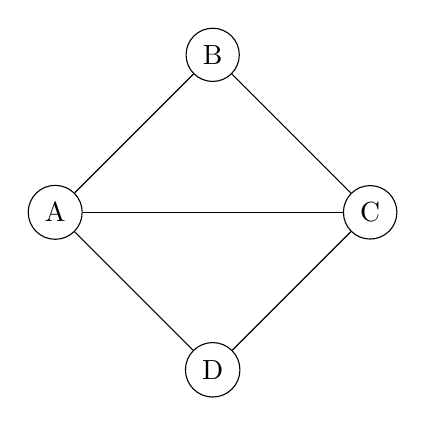
\begin{tikzpicture}
    % Define the vertices
    \node[circle,draw] (A) at (0,0) {A};
    \node[circle,draw] (B) at (2,2) {B};
    \node[circle,draw] (C) at (4,0) {C};
    \node[circle,draw] (D) at (2,-2) {D};

    % Draw the edges
    \draw (A) -- (B);
    \draw (B) -- (C);
    \draw (C) -- (D);
    \draw (D) -- (A);
    \draw (A) -- (C);
\end{tikzpicture}
%%

% برای تولید بخش مراجع از bibtex استفاده می‌شود. 
\bibliographystyle{plain-fa}
\bibliography{refs}

\pagestyle{empty}

% بخش مربوط به پیوست‌ها. اگر به این بخش نیاز ندارید می‌توانید این دستورات را کامنت کنید.
\appendixMode



\chapter{‌ فضاهای اندازه‌ها}

\section{مقدمه }


\chapter{‌  نامتناهی فضاهای اندازه‌ها}

% دستورات مربوط به تولید خودکار و چاپ نمایه در خروجی. نمایه به طور خودکار تولید می‌شود. اگر به این بخش نیاز ندارید می‌توانید این دستورات را کامنت کنید.
\includeIndex

%  دستورات مربوط به تولید خودکار و چاپ واژه‌نامهٔ انگلیسی به فارسی در خروجی. اگر به این بخش نیاز ندارید می‌توانید این دستورات را کامنت کنید.
\includeEntoFaDictionary

%  دستورات مربوط به تولید خودکار و چاپ واژه‌نامهٔ فارسی به انگلیسی در خروجی. اگر به این بخش نیاز ندارید می‌توانید این دستورات را کامنت کنید.
\includeFatoEnDictionary


%  در این بخش مقالات مستخرج از رساله/پایان‌نامه را در صورت وجود بیاورید. اگر به این بخش نیاز ندارید می‌توانید این دستورات را کامنت کنید.
\newpage
\section*{فهرست مقاله‌های مستخرج از پایان‌نامه/رساله}



\end{document}